\begin{figure*}

\definecolor{R}{rgb}{1,0,0} % red
\definecolor{G}{rgb}{0,0.6,0.36078431372} % forestgreen
\definecolor{B}{rgb}{0,0,1} % blue
\definecolor{O}{rgb}{0.99607843137,0.63529411764,0.22745098039} % orange
\definecolor{P}{rgb}{0.60784313725,0.27843137254,0.58823529411} % purple
\centering
% \newcommand{\uniquesize}{0.115\textwidth}
\newcommand{\uniquesize}{0.14\textwidth}
%
%
%
\begin{subfigure}[b]{\uniquesize}
\centering
\resizebox{!}{\textwidth}{
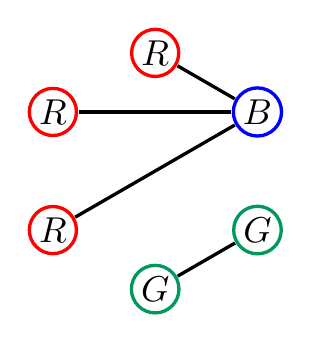
\begin{tikzpicture}[
mynode/.style={draw, circle, very thick, inner sep=1pt, scale=1.3},
myline/.style={draw, very thick},
]
\pgfmathsetmacro{\n}{6};
\pgfmathsetmacro{\r}{1.5};
\node[mynode,draw=R] (1) at (0*360/\n + 90: \r cm) {$\xcolor{R}$};
\node[mynode,draw=R] (2) at (1*360/\n + 90: \r cm) {$\xcolor{R}$};
\node[mynode,draw=R] (3) at (2*360/\n + 90: \r cm) {$\xcolor{R}$};
\node[mynode,draw=G] (4) at (3*360/\n + 90: \r cm) {$\xcolor{G}$};
\node[mynode,draw=G] (5) at (4*360/\n + 90: \r cm) {$\xcolor{G}$};
\node[mynode,draw=B] (6) at (5*360/\n + 90: \r cm) {$\xcolor{B}$};
\draw [myline] (6) -- (1);
\draw [myline] (6) -- (2);
\draw [myline] (6) -- (3);
\draw [myline] (5) -- (4);
\end{tikzpicture}
}
\caption{\mypm{}~227}
\end{subfigure}
%
%
%
\begin{subfigure}[b]{\uniquesize}
\centering
\resizebox{!}{\textwidth}{
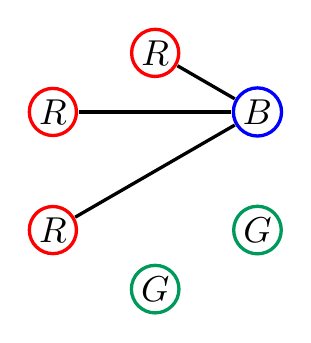
\begin{tikzpicture}[
mynode/.style={draw, circle, very thick, inner sep=1pt, scale=1.3},
myline/.style={draw, very thick},
]
\pgfmathsetmacro{\n}{6};
\pgfmathsetmacro{\r}{1.5};
\node[mynode,draw=R] (1) at (0*360/\n + 90: \r cm) {$\xcolor{R}$};
\node[mynode,draw=R] (2) at (1*360/\n + 90: \r cm) {$\xcolor{R}$};
\node[mynode,draw=R] (3) at (2*360/\n + 90: \r cm) {$\xcolor{R}$};
\node[mynode,draw=G] (4) at (3*360/\n + 90: \r cm) {$\xcolor{G}$};
\node[mynode,draw=G] (5) at (4*360/\n + 90: \r cm) {$\xcolor{G}$};
\node[mynode,draw=B] (6) at (5*360/\n + 90: \r cm) {$\xcolor{B}$};
\draw [myline] (6) -- (1);
\draw [myline] (6) -- (2);
\draw [myline] (6) -- (3);
\end{tikzpicture}
}
\caption{\mypm{}~228}
\end{subfigure}
%
%
%
\begin{subfigure}[b]{\uniquesize}
\centering
\resizebox{!}{\textwidth}{
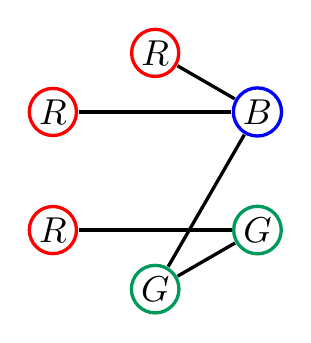
\begin{tikzpicture}[
mynode/.style={draw, circle, very thick, inner sep=1pt, scale=1.3},
myline/.style={draw, very thick},
]
\pgfmathsetmacro{\n}{6};
\pgfmathsetmacro{\r}{1.5};
\node[mynode,draw=R] (1) at (0*360/\n + 90: \r cm) {$\xcolor{R}$};
\node[mynode,draw=R] (2) at (1*360/\n + 90: \r cm) {$\xcolor{R}$};
\node[mynode,draw=R] (3) at (2*360/\n + 90: \r cm) {$\xcolor{R}$};
\node[mynode,draw=G] (4) at (3*360/\n + 90: \r cm) {$\xcolor{G}$};
\node[mynode,draw=G] (5) at (4*360/\n + 90: \r cm) {$\xcolor{G}$};
\node[mynode,draw=B] (6) at (5*360/\n + 90: \r cm) {$\xcolor{B}$};
\draw [myline] (6) -- (1);
\draw [myline] (6) -- (2);
\draw [myline] (5) -- (3);
\draw [myline] (5) -- (4);
\draw [myline] (6) -- (4);
\end{tikzpicture}
}
\caption{\mypm{}~332}
\end{subfigure}
%
%
%
\begin{subfigure}[b]{\uniquesize}
\centering
\resizebox{!}{\textwidth}{
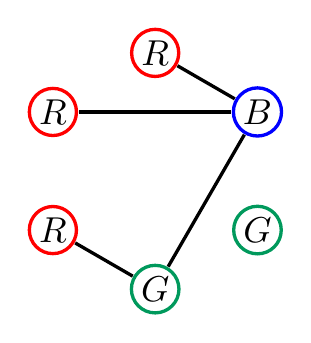
\begin{tikzpicture}[
mynode/.style={draw, circle, very thick, inner sep=1pt, scale=1.3},
myline/.style={draw, very thick},
]
\pgfmathsetmacro{\n}{6};
\pgfmathsetmacro{\r}{1.5};
\node[mynode,draw=R] (1) at (0*360/\n + 90: \r cm) {$\xcolor{R}$};
\node[mynode,draw=R] (2) at (1*360/\n + 90: \r cm) {$\xcolor{R}$};
\node[mynode,draw=R] (3) at (2*360/\n + 90: \r cm) {$\xcolor{R}$};
\node[mynode,draw=G] (4) at (3*360/\n + 90: \r cm) {$\xcolor{G}$};
\node[mynode,draw=G] (5) at (4*360/\n + 90: \r cm) {$\xcolor{G}$};
\node[mynode,draw=B] (6) at (5*360/\n + 90: \r cm) {$\xcolor{B}$};
\draw [myline] (6) -- (1);
\draw [myline] (6) -- (2);
\draw [myline] (4) -- (3);
\draw [myline] (6) -- (4);
\end{tikzpicture}
}
\caption{\mypm{}~438}
\end{subfigure}
%
%
%
\begin{subfigure}[b]{\uniquesize}
\centering
\resizebox{!}{\textwidth}{
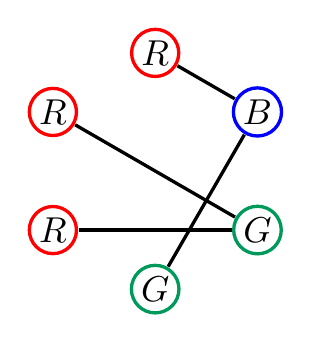
\begin{tikzpicture}[
mynode/.style={draw, circle, very thick, inner sep=1pt, scale=1.3},
myline/.style={draw, very thick},
]
\pgfmathsetmacro{\n}{6};
\pgfmathsetmacro{\r}{1.5};
\node[mynode,draw=R] (1) at (0*360/\n + 90: \r cm) {$\xcolor{R}$};
\node[mynode,draw=R] (2) at (1*360/\n + 90: \r cm) {$\xcolor{R}$};
\node[mynode,draw=R] (3) at (2*360/\n + 90: \r cm) {$\xcolor{R}$};
\node[mynode,draw=G] (4) at (3*360/\n + 90: \r cm) {$\xcolor{G}$};
\node[mynode,draw=G] (5) at (4*360/\n + 90: \r cm) {$\xcolor{G}$};
\node[mynode,draw=B] (6) at (5*360/\n + 90: \r cm) {$\xcolor{B}$};
\draw [myline] (6) -- (1);
\draw [myline] (5) -- (2);
\draw [myline] (5) -- (3);
\draw [myline] (6) -- (4);
\end{tikzpicture}
}
\caption{\mypm{}~467}
\end{subfigure}
%
%
%
\begin{subfigure}[b]{\uniquesize}
\centering
\resizebox{!}{\textwidth}{
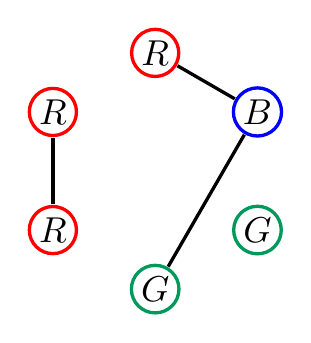
\begin{tikzpicture}[
mynode/.style={draw, circle, very thick, inner sep=1pt, scale=1.3},
myline/.style={draw, very thick},
]
\pgfmathsetmacro{\n}{6};
\pgfmathsetmacro{\r}{1.5};
\node[mynode,draw=R] (1) at (0*360/\n + 90: \r cm) {$\xcolor{R}$};
\node[mynode,draw=R] (2) at (1*360/\n + 90: \r cm) {$\xcolor{R}$};
\node[mynode,draw=R] (3) at (2*360/\n + 90: \r cm) {$\xcolor{R}$};
\node[mynode,draw=G] (4) at (3*360/\n + 90: \r cm) {$\xcolor{G}$};
\node[mynode,draw=G] (5) at (4*360/\n + 90: \r cm) {$\xcolor{G}$};
\node[mynode,draw=B] (6) at (5*360/\n + 90: \r cm) {$\xcolor{B}$};
\draw [myline] (6) -- (1);
\draw [myline] (3) -- (2);
\draw [myline] (6) -- (4);
\end{tikzpicture}
}
\caption{\mypm{}~468}
\end{subfigure}
%
%
%
\begin{subfigure}[b]{\uniquesize}
\centering
\resizebox{!}{\textwidth}{
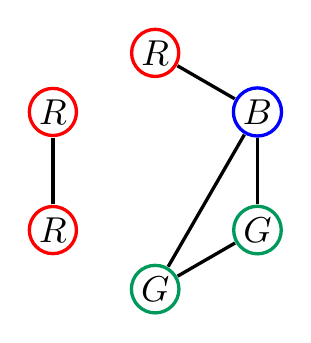
\begin{tikzpicture}[
mynode/.style={draw, circle, very thick, inner sep=1pt, scale=1.3},
myline/.style={draw, very thick},
]
\pgfmathsetmacro{\n}{6};
\pgfmathsetmacro{\r}{1.5};
\node[mynode,draw=R] (1) at (0*360/\n + 90: \r cm) {$\xcolor{R}$};
\node[mynode,draw=R] (2) at (1*360/\n + 90: \r cm) {$\xcolor{R}$};
\node[mynode,draw=R] (3) at (2*360/\n + 90: \r cm) {$\xcolor{R}$};
\node[mynode,draw=G] (4) at (3*360/\n + 90: \r cm) {$\xcolor{G}$};
\node[mynode,draw=G] (5) at (4*360/\n + 90: \r cm) {$\xcolor{G}$};
\node[mynode,draw=B] (6) at (5*360/\n + 90: \r cm) {$\xcolor{B}$};
\draw [myline] (6) -- (1);
\draw [myline] (3) -- (2);
\draw [myline] (5) -- (4);
\draw [myline] (6) -- (4);
\draw [myline] (6) -- (5);
\end{tikzpicture}
}
\caption{\mypm{}~678\label{fig:ch2:unique1:g}}
\end{subfigure}
%
%
%
\begin{subfigure}[b]{\uniquesize}
\centering
\resizebox{!}{\textwidth}{
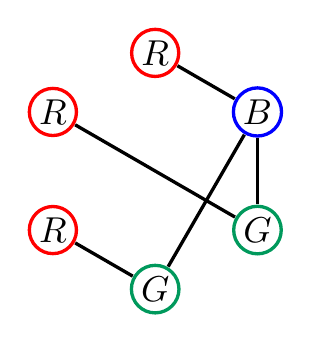
\begin{tikzpicture}[
mynode/.style={draw, circle, very thick, inner sep=1pt, scale=1.3},
myline/.style={draw, very thick},
]
\pgfmathsetmacro{\n}{6};
\pgfmathsetmacro{\r}{1.5};
\node[mynode,draw=R] (1) at (0*360/\n + 90: \r cm) {$\xcolor{R}$};
\node[mynode,draw=R] (2) at (1*360/\n + 90: \r cm) {$\xcolor{R}$};
\node[mynode,draw=R] (3) at (2*360/\n + 90: \r cm) {$\xcolor{R}$};
\node[mynode,draw=G] (4) at (3*360/\n + 90: \r cm) {$\xcolor{G}$};
\node[mynode,draw=G] (5) at (4*360/\n + 90: \r cm) {$\xcolor{G}$};
\node[mynode,draw=B] (6) at (5*360/\n + 90: \r cm) {$\xcolor{B}$};
\draw [myline] (6) -- (1);
\draw [myline] (5) -- (2);
\draw [myline] (4) -- (3);
\draw [myline] (6) -- (4);
\draw [myline] (6) -- (5);
\end{tikzpicture}
}
\caption{\mypm{}~691}
\end{subfigure}
%
%
%
\begin{subfigure}[b]{\uniquesize}
\centering
\resizebox{!}{\textwidth}{
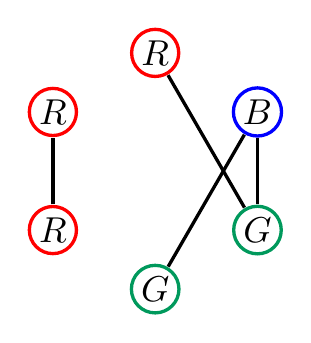
\begin{tikzpicture}[
mynode/.style={draw, circle, very thick, inner sep=1pt, scale=1.3},
myline/.style={draw, very thick},
]
\pgfmathsetmacro{\n}{6};
\pgfmathsetmacro{\r}{1.5};
\node[mynode,draw=R] (1) at (0*360/\n + 90: \r cm) {$\xcolor{R}$};
\node[mynode,draw=R] (2) at (1*360/\n + 90: \r cm) {$\xcolor{R}$};
\node[mynode,draw=R] (3) at (2*360/\n + 90: \r cm) {$\xcolor{R}$};
\node[mynode,draw=G] (4) at (3*360/\n + 90: \r cm) {$\xcolor{G}$};
\node[mynode,draw=G] (5) at (4*360/\n + 90: \r cm) {$\xcolor{G}$};
\node[mynode,draw=B] (6) at (5*360/\n + 90: \r cm) {$\xcolor{B}$};
\draw [myline] (5) -- (1);
\draw [myline] (3) -- (2);
\draw [myline] (6) -- (4);
\draw [myline] (6) -- (5);
\end{tikzpicture}
}
\caption{\mypm{}~700}
\end{subfigure}
%
%
%
\begin{subfigure}[b]{\uniquesize}
\centering
\resizebox{!}{\textwidth}{
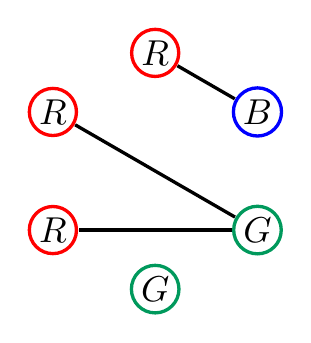
\begin{tikzpicture}[
mynode/.style={draw, circle, very thick, inner sep=1pt, scale=1.3},
myline/.style={draw, very thick},
]
\pgfmathsetmacro{\n}{6};
\pgfmathsetmacro{\r}{1.5};
\node[mynode,draw=R] (1) at (0*360/\n + 90: \r cm) {$\xcolor{R}$};
\node[mynode,draw=R] (2) at (1*360/\n + 90: \r cm) {$\xcolor{R}$};
\node[mynode,draw=R] (3) at (2*360/\n + 90: \r cm) {$\xcolor{R}$};
\node[mynode,draw=G] (4) at (3*360/\n + 90: \r cm) {$\xcolor{G}$};
\node[mynode,draw=G] (5) at (4*360/\n + 90: \r cm) {$\xcolor{G}$};
\node[mynode,draw=B] (6) at (5*360/\n + 90: \r cm) {$\xcolor{B}$};
\draw [myline] (6) -- (1);
\draw [myline] (5) -- (2);
\draw [myline] (5) -- (3);
\end{tikzpicture}
}
\caption{\mypm{}~844}
\end{subfigure}
%
%
%
\begin{subfigure}[b]{\uniquesize}
\centering
\resizebox{!}{\textwidth}{
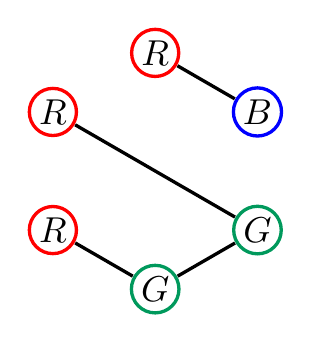
\begin{tikzpicture}[
mynode/.style={draw, circle, very thick, inner sep=1pt, scale=1.3},
myline/.style={draw, very thick},
]
\pgfmathsetmacro{\n}{6};
\pgfmathsetmacro{\r}{1.5};
\node[mynode,draw=R] (1) at (0*360/\n + 90: \r cm) {$\xcolor{R}$};
\node[mynode,draw=R] (2) at (1*360/\n + 90: \r cm) {$\xcolor{R}$};
\node[mynode,draw=R] (3) at (2*360/\n + 90: \r cm) {$\xcolor{R}$};
\node[mynode,draw=G] (4) at (3*360/\n + 90: \r cm) {$\xcolor{G}$};
\node[mynode,draw=G] (5) at (4*360/\n + 90: \r cm) {$\xcolor{G}$};
\node[mynode,draw=B] (6) at (5*360/\n + 90: \r cm) {$\xcolor{B}$};
\draw [myline] (6) -- (1);
\draw [myline] (5) -- (2);
\draw [myline] (4) -- (3);
\draw [myline] (5) -- (4);
\end{tikzpicture}
}
\caption{\mypm{}~850}
\end{subfigure}
%
%
%
\begin{subfigure}[b]{\uniquesize}
\centering
\resizebox{!}{\textwidth}{
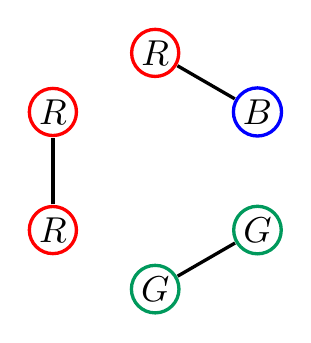
\begin{tikzpicture}[
mynode/.style={draw, circle, very thick, inner sep=1pt, scale=1.3},
myline/.style={draw, very thick},
]
\pgfmathsetmacro{\n}{6};
\pgfmathsetmacro{\r}{1.5};
\node[mynode,draw=R] (1) at (0*360/\n + 90: \r cm) {$\xcolor{R}$};
\node[mynode,draw=R] (2) at (1*360/\n + 90: \r cm) {$\xcolor{R}$};
\node[mynode,draw=R] (3) at (2*360/\n + 90: \r cm) {$\xcolor{R}$};
\node[mynode,draw=G] (4) at (3*360/\n + 90: \r cm) {$\xcolor{G}$};
\node[mynode,draw=G] (5) at (4*360/\n + 90: \r cm) {$\xcolor{G}$};
\node[mynode,draw=B] (6) at (5*360/\n + 90: \r cm) {$\xcolor{B}$};
\draw [myline] (6) -- (1);
\draw [myline] (3) -- (2);
\draw [myline] (5) -- (4);
\end{tikzpicture}
}
\caption{\mypm{}~852}
\end{subfigure}
%
%
%
\begin{subfigure}[b]{\uniquesize}
\centering
\resizebox{!}{\textwidth}{
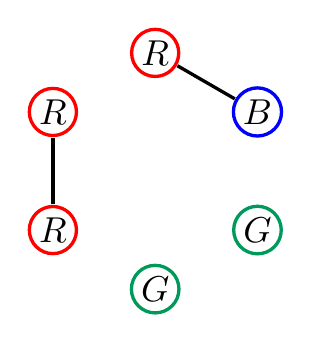
\begin{tikzpicture}[
mynode/.style={draw, circle, very thick, inner sep=1pt, scale=1.3},
myline/.style={draw, very thick},
]
\pgfmathsetmacro{\n}{6};
\pgfmathsetmacro{\r}{1.5};
\node[mynode,draw=R] (1) at (0*360/\n + 90: \r cm) {$\xcolor{R}$};
\node[mynode,draw=R] (2) at (1*360/\n + 90: \r cm) {$\xcolor{R}$};
\node[mynode,draw=R] (3) at (2*360/\n + 90: \r cm) {$\xcolor{R}$};
\node[mynode,draw=G] (4) at (3*360/\n + 90: \r cm) {$\xcolor{G}$};
\node[mynode,draw=G] (5) at (4*360/\n + 90: \r cm) {$\xcolor{G}$};
\node[mynode,draw=B] (6) at (5*360/\n + 90: \r cm) {$\xcolor{B}$};
\draw [myline] (6) -- (1);
\draw [myline] (3) -- (2);
\end{tikzpicture}
}
\caption{\mypm{}~855}
\end{subfigure}
%
%
%
\begin{subfigure}[b]{\uniquesize}
\centering
\resizebox{!}{\textwidth}{
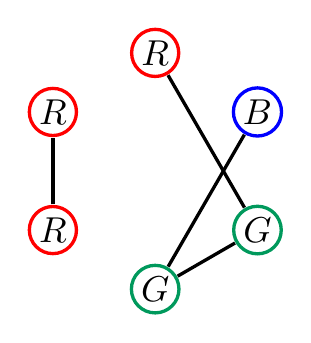
\begin{tikzpicture}[
mynode/.style={draw, circle, very thick, inner sep=1pt, scale=1.3},
myline/.style={draw, very thick},
]
\pgfmathsetmacro{\n}{6};
\pgfmathsetmacro{\r}{1.5};
\node[mynode,draw=R] (1) at (0*360/\n + 90: \r cm) {$\xcolor{R}$};
\node[mynode,draw=R] (2) at (1*360/\n + 90: \r cm) {$\xcolor{R}$};
\node[mynode,draw=R] (3) at (2*360/\n + 90: \r cm) {$\xcolor{R}$};
\node[mynode,draw=G] (4) at (3*360/\n + 90: \r cm) {$\xcolor{G}$};
\node[mynode,draw=G] (5) at (4*360/\n + 90: \r cm) {$\xcolor{G}$};
\node[mynode,draw=B] (6) at (5*360/\n + 90: \r cm) {$\xcolor{B}$};
\draw [myline] (5) -- (1);
\draw [myline] (3) -- (2);
\draw [myline] (5) -- (4);
\draw [myline] (6) -- (4);
\end{tikzpicture}
}
\caption{\mypm{}~895}
\end{subfigure}
%
%
%
\begin{subfigure}[b]{\uniquesize}
\centering
\resizebox{!}{\textwidth}{
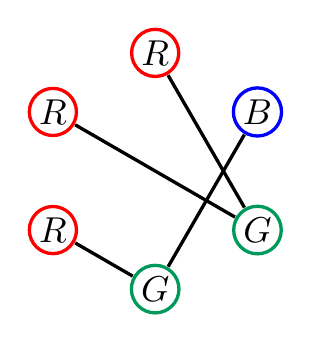
\begin{tikzpicture}[
mynode/.style={draw, circle, very thick, inner sep=1pt, scale=1.3},
myline/.style={draw, very thick},
]
\pgfmathsetmacro{\n}{6};
\pgfmathsetmacro{\r}{1.5};
\node[mynode,draw=R] (1) at (0*360/\n + 90: \r cm) {$\xcolor{R}$};
\node[mynode,draw=R] (2) at (1*360/\n + 90: \r cm) {$\xcolor{R}$};
\node[mynode,draw=R] (3) at (2*360/\n + 90: \r cm) {$\xcolor{R}$};
\node[mynode,draw=G] (4) at (3*360/\n + 90: \r cm) {$\xcolor{G}$};
\node[mynode,draw=G] (5) at (4*360/\n + 90: \r cm) {$\xcolor{G}$};
\node[mynode,draw=B] (6) at (5*360/\n + 90: \r cm) {$\xcolor{B}$};
\draw [myline] (5) -- (1);
\draw [myline] (5) -- (2);
\draw [myline] (4) -- (3);
\draw [myline] (6) -- (4);
\end{tikzpicture}
}
\caption{\mypm{}~904}
\end{subfigure}
%
%
%
\begin{subfigure}[b]{\uniquesize}
\centering
\resizebox{!}{\textwidth}{
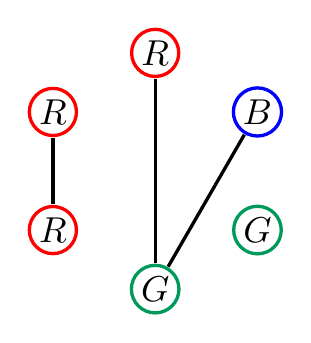
\begin{tikzpicture}[
mynode/.style={draw, circle, very thick, inner sep=1pt, scale=1.3},
myline/.style={draw, very thick},
]
\pgfmathsetmacro{\n}{6};
\pgfmathsetmacro{\r}{1.5};
\node[mynode,draw=R] (1) at (0*360/\n + 90: \r cm) {$\xcolor{R}$};
\node[mynode,draw=R] (2) at (1*360/\n + 90: \r cm) {$\xcolor{R}$};
\node[mynode,draw=R] (3) at (2*360/\n + 90: \r cm) {$\xcolor{R}$};
\node[mynode,draw=G] (4) at (3*360/\n + 90: \r cm) {$\xcolor{G}$};
\node[mynode,draw=G] (5) at (4*360/\n + 90: \r cm) {$\xcolor{G}$};
\node[mynode,draw=B] (6) at (5*360/\n + 90: \r cm) {$\xcolor{B}$};
\draw [myline] (4) -- (1);
\draw [myline] (3) -- (2);
\draw [myline] (6) -- (4);
\end{tikzpicture}
}
\caption{\mypm{}~913}
\end{subfigure}
%
%
%

\caption{All 16 unique graphs with no additional NSCs for \nameref{sec:ch2:example1}. \label{fig:ch2:unique1}}

\end{figure*}